% !TeX root = ../main.tex
% Add the above to each chapter to make compiling the PDF easier in some editors.

\chapter{Background}\label{chapter:background}
\section{Related Works}


Robot manipulation and grasping is an intensively researched area. The wide span of the subject makes it hard to categorize all different approaches under one umbrella. Nevertheless, analytical and empirical grasping approaches tend to be the most used categorization in the literature \cite{Sahbani2012}.  


\subsection{Analytical Grasping Approach}

The analytical approach has been introduced first by Nguyen. He tries to solve the grasping problem by defining analytical objectives. Such as a successful grasp should achieve force closure and satisfy the stability conditions by closing the object from each direction \cite{Nguyen1987}. Nguyen models the hand and the object, to be grasped, to compute the stable force closure grasp analytically. This kind of analytical techniques comes with an exhaustive computation burden. Although the proposed algorithm works fast and correct when the object is planar and flat with a small number of faces, they don’t scale to household objects such as mugs or bottles \cite{Sahbani2012}. Moreover, in most robotics setups full geometrical models of the objects are not available \cite{Schmidt2018}. 

\begin{figure}

    \begin{subfigure}{0.31\textwidth}
      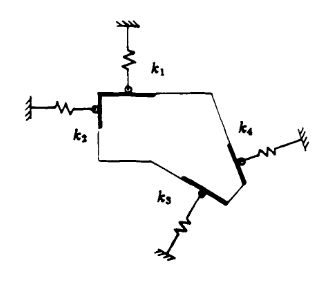
\includegraphics[width=\linewidth]{figures/graspA.png}
      \caption{} \label{fig:1a}
    \end{subfigure}%
    \hspace*{\fill}   % maximize separation between the subfigures
    \begin{subfigure}{0.31\textwidth}
      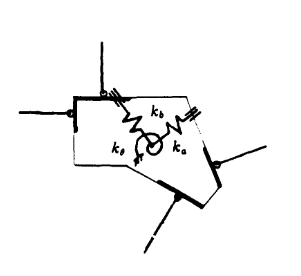
\includegraphics[width=\linewidth]{figures/graspB.png}
      \caption{} \label{fig:1b}
    \end{subfigure}%
    \hspace*{\fill}   % maximizeseparation between the subfigures
    \begin{subfigure}{0.31\textwidth}
      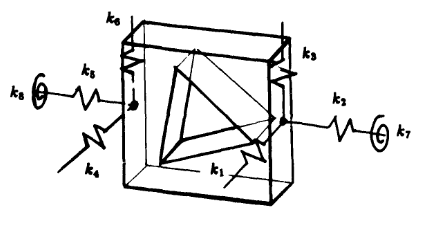
\includegraphics[width=\linewidth]{figures/graspC.png}
      \caption{} \label{fig:1c}
    \end{subfigure}

\caption{Stable force closure examples fingers are represented as virtual springs. Nguyen proved that all force closures can modified to be a stable grasp candidate\cite{Nguyen1987}.} \label{fig:1}
\end{figure}

\subsection{Empirical Grasping Approach}


The empirical grasping approach introduced to overcome the difficulties faced with the analytical grasping approach. Empirical methods include learning, which is based on sampling and then training. Some examples of empirical grasping approaches are imitating a human teacher \cite{Ekvall2004}, learning from the handcrafted features \cite{Saxena2008},  and deep reinforcement learning(RL) technique to learn close-loop dynamic visual grasping strategies \cite{Kalashnikov2018}. Imitating a human teacher can easily learn the demonstrated training data. However, it has difficulties to scale to the novel objects, which were not seen during the training \cite{Sahbani2012}. Saxena et al.’s technique to learn from the feature effectively generalize to unseen objects but it fails to choose the best grasp for a particular task \cite{Sahbani2012}. RL approaches learn a particular grasp of an object based on a definition of a goal. Thus, the learned grasp of an object already linked to the task's goal. The flexibility of RL made itself attractive among grasping researchers. One disadvantage of the RL approach is that, it requires a considerable amount of data to train. Although recent applications introduced randomization for sim-to-real transfer of the models \cite{Andrychowicz2020}, it still has difficulties to perform reliably in the real-world \cite{Caldera2018}.

\section{Learning applications on grasping}

Experts implement handcrafted features and hand-coded controllers. Thus, it is time-consuming and incapable of generalizing to new objects and scenery. Among all other approaches, machine learning applications on grasping has proven to give a high success rate on novel objects.


\subsection{Deep Learning for Detecting Grasps candidates}
Lenz et al. propose a five parameters model trained by supervised learning from the candidate grasps database. They draw a rectangle box representing the best grasp location with the five-dimensional parameter model, x, y coordinates, width, height, and orientation.

Their cascaded network architecture bypasses the need for a handcrafted features. After training, the first layer network learns low-level features and delivers possible naïve grasping candidates, and the second layer chooses the top-ranked grasping candidate \ref{fig:deeplearngrasp}.

Although they achieved up to \(90\%\) success rate on grasping Lab tools, this method is limited to only parallel plate gripper. When one wants to use another gripper type, the dataset should be updated entirely for that gripper. Besides data collection process is time-consuming and biased

\begin{figure}[htbp]
    \centering
    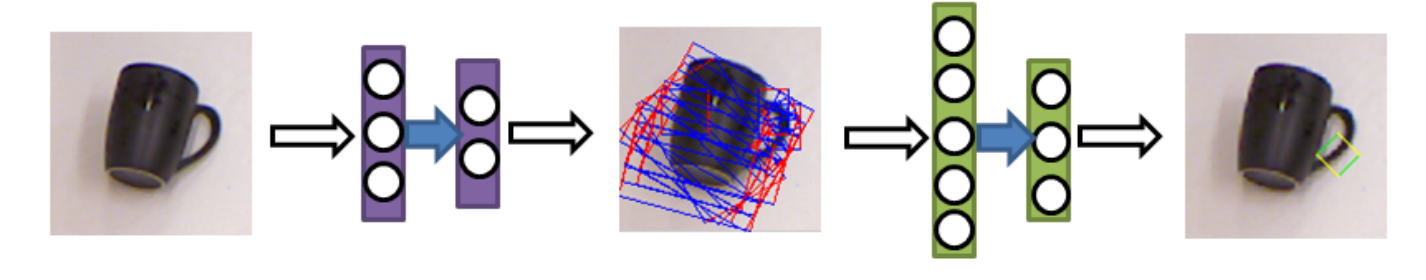
\includegraphics[width=1.\textwidth]{figures/DeepLearningGrasp}
    \caption{Red-blue rectangles represent possible grasp candidate. Green rectangle is the top-ranked grasp rectangle \cite{Lenz2013}}
    \label{fig:deeplearngrasp}
\end{figure}

\subsection{Dex-net}
\todo{Architectur'i anlat. Robustness factor nasil parametirize edildi?}

Another approach for grasping is to learn the grasp robustness factor. Mahlet etal  trained convolutional neural networks to learn the grasps robustness function from 6.7 million point cloud data. They collect the data similarly to Lenz et al. with an analytical grasp metric to evaluate the quality of a grasp. 

\begin{figure}[htbp]
    \centering
    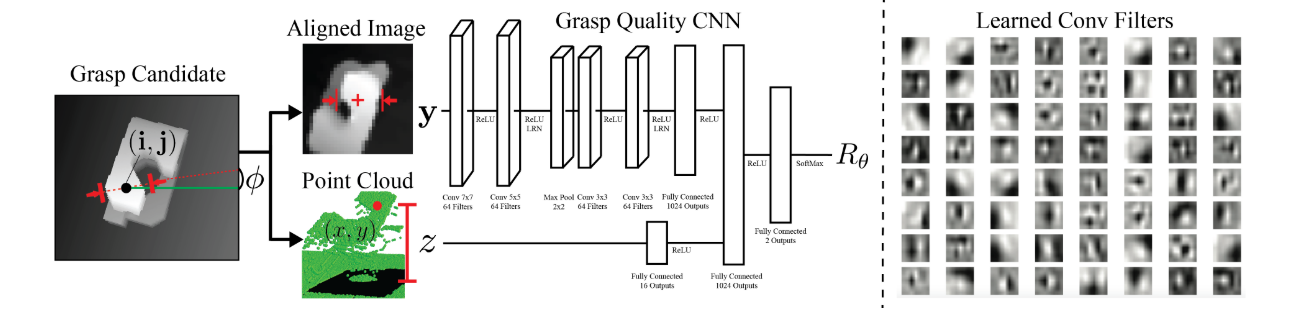
\includegraphics[width=1.\textwidth]{figures/dexnet}
    \caption{Dex-net architecture \cite{Lenz2013}}
    \label{fig:dexnet}
\end{figure}

With \(98\%\) success rate, their approach indeed proved to be robust. However, the designed network only outputs the grasp location such that a grasp planning algorithm is needed to complete the grasping process. Moreover, data collection can be tedious due to a large number of a machine-labeled dataset.


\subsection{Deep Reinforcement Learning for Vision-Based Robotic Grasping: A Simulated Comparative Evaluation of Off-Policy Methods}

The sequential decision-making process is inherent in all grasp tasks. This property of grasping helps us to model it with a reinforcement learning framework. Unlike other works, this approach trains end-to-end policies to automatically learn to grasp without any prior knowledge about the environment or the gripper model. Moreover, the end-to-end nature of their system eliminates the need for additional grasp planner, which was a default in previous works. 
Quillen et al. show that off-policy RL can increase the robustness of grasping models. Based on their investigation, corrected Monte Carlo and Deep Q Learning outperform the earlier supervised learning approach. They observe that model-free RL approaches allow pre-grasp manipulation to increase the chances of grasp in future actions. 

\begin{figure}[htbp]
    \centering
    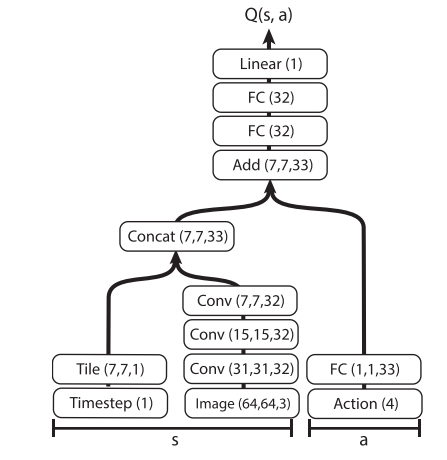
\includegraphics[width=0.5\textwidth]{figures/dql}
    \caption{Deep Learning network architecture of \cite{Quillen2018}}
    \label{fig:dql}
\end{figure}

They suit one complete network to concatenate perception input and actions from two different branches \ref{fig:dql}. Although the number of parameters increases drastically with convolutional layers from the perception branch, it makes the system more compact and easier to understand.

\subsection{Comparing Task Simplifications to Learn Closed-Loop Object Picking Using Deep Reinforcement Learning}

The learning setup is similar to the Quillen et al. with one robot gripper and randomly spawned objects in the simulation. One significant difference regarding the learning setup is Breyer et al. generates the robot gripper only until the wrist without the rest of the arm and, therefore, doesn’t need to calculate the inverse kinematics equation.

Breyer et al. enhanced the RL based data-driven grasp approach with Curriculum Learning and the introduction of auto-encoder for perception. Thanks to the curriculum learning setup, which increases the task difficulty based on the agent’s current performance, they shortened the time for the agent to explore the environment. In other words, curriculum learning guides the agent throughout its learning phase. Besides, with the help of autoencoder for the perception layer, their network tends to spend less time to comprehend the observation compare to the Quillen et al.’s approach. 

Unlike Quillen et al., they experimented with policy-based on-policy RL algorithm, TRPO. Policy -based algorithms tend to 
\todo{Policy based vs. value based here not exploration }
explore better than epsilon greedy based exploration. This property may also contribute to the higher success rate and faster convergence. After training grasping models on simulation, they tested them on a real robot. Although they didn’t use domain randomization to minimize the reality gap, they achieved up to \(78\%\) success rate.

\begin{figure}[htbp]
    \centering
    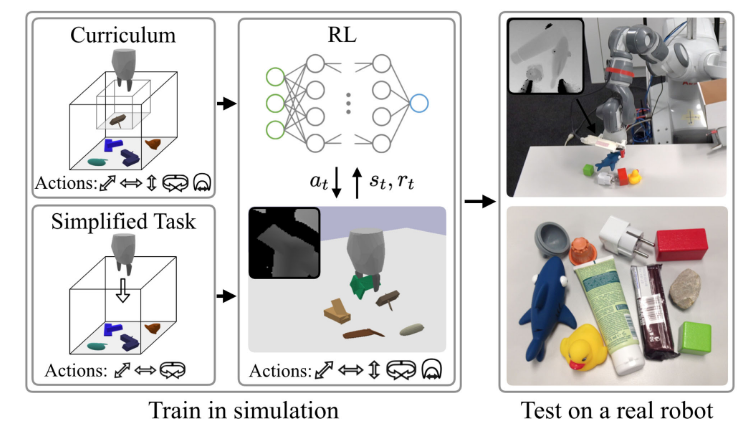
\includegraphics[width=0.7\textwidth]{figures/curriculum}
    \caption{Breyer et al. \cite{Breyer2018}}
    \label{fig:dql}
\end{figure}


\subsection{Solving Rubik's Cube With a Robot Hand}

OpenAI et al. present a novel approach for in-hand manipulation problems. Their system attacks Sim2Real discrepancy between simulated models performing on real robots. 

Training the Deep RL models on simulation is becoming more and more common. The popularity of simulation increases the demand for enhanced Sim2Real model transfer algorithms. Domain randomization has shown great success in bridging the gap between reality and simulation \cite{Tobin2017}. More researchers implement machine learning methods that randomize the environment and gripper material parameters. Through this approach, trained models can achieve higher generalization property with robustness to increasing noise on the sensor or environment settings.
OpenAI proposes a Meta-Learning method with policies that involve memory like recurrent neural networks that can learn the underlying dynamics of the environment—combining meta-learning with automated domain randomization algorithm results on an enhanced adaptation of models on real-world robots.

\begin{figure}[htbp]
    \centering
    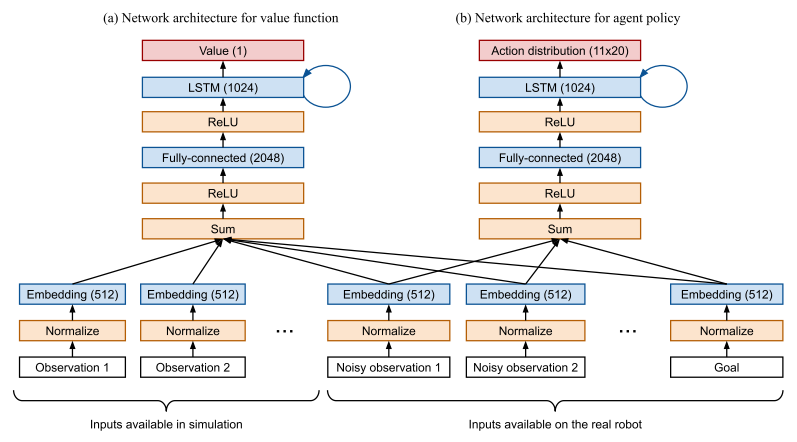
\includegraphics[width=1.\textwidth]{figures/openai}
    \caption{OpenAI policy and value network architecture \cite{openai2019rubiks}}
    \label{fig:dql}
\end{figure}


% !TeX root = ../main.tex
% Add the above to each chapter to make compiling the PDF easier in some editors.

\section{Reinforcement Learning}

The simplest examples of learning come from our own life; we learn to walk, speak the language, or to cook. All those activities span our entire life, it influences who we are and the decisions we take in life. We know that living animals such as mammals learn from their social and asocial interactions with the environment.
We know that living animals such as mammals learn from their social and asocial interactions with the environment \cite{AnimalInt11}. 
Although we have not yet developed a full-scale theory of animal learning, we have developed computational objectives for machines to learn \cite{Sutton2018}. 
This computational approach can be categorized as Supervised, Unsupervised or Reinforcement Learning. This computational approach falls into three categories as Supervised, Unsupervised, or Reinforcement Learning.

In this chapter, we will consider the Reinforcement Learning objectives and problem formulation.
Reinforcement Learning provides a systematic approach to maximize the reward by linking observations to actions. A reinforcement learning agent creates its data by interacting with the environment. Therefore, it is fundamentally different from supervised and unsupervised learning, where the data is already provided \cite{Sutton2018}. 
Another important difference is the inherent goal-oriented approach. Reinforcement learning agent maximizes the rewards for its inherent general goal. Other machine learning approaches lack this goal \cite{Sutton2018}.
For instance, supervised learned software recognizing faces can be used for security reasons to detect criminals or can be easily used to unlock phones. However, a reinforcement learning agent trained to drive a car autonomously can only drive a car. In a sense, reinforcement learning provides us end-to-end learning.

A core feature of reinforcement learning is that it acts on uncertain environments and, in return, receives the observation and reward. Fundamentally, a learning agent collects this experience and tunes its action to increase the expected reward. The expected reward term refers to the end of the horizon. For example, a chess-playing agent can choose to sacrifice the queen in the next move for a checkmate in the move after. In this case, the reward would decrease when the agent loses a queen, but the goal of the agent will be satisfied by terminating the game. For a well-defined reinforcement learning system, we can speak of four main components: Policy to decide the actions, a reward to maximize the expected reward in the horizon, and a model of the environment, telling which directions the chess pieces can move. The components of reinforcement learning are formulated based on Markov Decision Process. In the MDP chapter, we will detailly explain RL components. In the next chapters first Markov Chains, the simple version of MDP, then MDP, the slightly advanced version of Markov Chains, will be explained by some simple modifications \cite{PerezMIT}.

\subsection{Markov Chain}

The weak law of large numbers has a tremendous significance on stochastic modeling. This law states that the average of a large number of experimentations converges to the real value of the probability of a particular task. As an example, if one tosses infinite amounts of the coin, the average number of heads should converge to 0.5 \cite{Gagniuc2017}. 
Bernoulli’s weak law of large numbers only covers independent events. Markov proved that Bernoulli’s law also holds on dependent cases \cite{Gagniuc2017}. 
As the law of large numbers suggests, if one conducts a large number of iterations on this problem, one can deduce the transition matrix. This matrix proves to be the only information one needs to compute the next state.
This characteristic defines the famous Markov property; the current state captures all the necessary information one needs to predict the next state. If we extrapolate this example to slightly complex systems, for example, weather forecast, we just need today’s weather report to predict tomorrow’s forecast, assuming that we know the transition matrix. Naturally, one can formulate other events with Markov Chain lawnmower, and random walk are the straightforward ones in the literature\cite{Gagniuc2017}.

It is also possible to attach rewards to Markov Chain’s formulation. In figure \ref{fig: markov_chain}, the transition between states is represented with the arcs. And each transition has a probability similar to the transition matrix; we defined before. Each state has an immediate reward and a value function. The immediate reward is received directly when the actor moves to that state. The value of a state represents how likely the future actor will end up collecting high rewards. 

\begin{figure}[htbp]
    \centering
    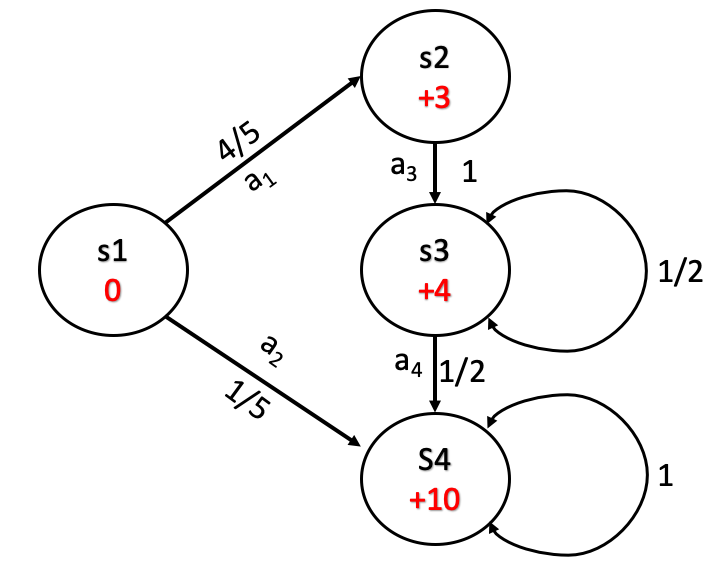
\includegraphics[width=0.5\textwidth]{figures/markovchain}
    \caption{Markov chain with transition probabilties and rewards}
    \label{fig: markov_chain}
\end{figure}

The value of a state will be later significant to solve Reinforcement Learning problems through Value Iteration methods. They are one of the essential algorithms that led to the initial success of Reinforcement Learning research.

    \subsection{Markov Decision Process}\label{section:markov}

Markov decision process is a slightly advanced version of the Markov Chain. It includes action on top of the Markov Chain. Reinforcement learning problems are formalized as a Markov Decision Process rather than Markov Chain because RL agents are free to choose from different actions.

MDPs first came into play as part of optimal control problem by Bellman \cite{Bellman1958}. Bellman applied dynamic programming methods to solve the MDP problem optimally. However, this methodology was not scalable to larger problems stem from the curse of dimensionality problem \cite{Sutton}.

The fundamental elements of MDP are as follows:
\begin{itemize}
    \item Agent:  The actor takes action on the environment to learn.
    \item Environment: The agent interacts with the Environment(Plant).
    \item Rewards: Environment returns rewards based on the interaction made by the actor.
    \item State: View of the environment from the eyes of the actor. 
\end{itemize}

\begin{figure}[htbp]
    \centering
    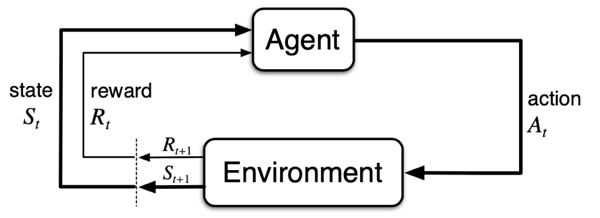
\includegraphics[width=0.8\textwidth]{figures/mdp}
    \caption{MDP structure}
    \label{fig: mdp}
\end{figure}

The process of action follows; the agent acts on the environment at time t and environment return the reward and state of the action at time \(t+1\). Based on the state of the environment at the \(t+1\) agent makes another action \(A_{t+1}\), which results in \(R_{t+2}\) and \(S_{t+2}\).

In every MDP system, agents should be reachable to every state through a sequence of actions. The transition between states is of great value for the MDP framework.
One can compute the transition probability in MDP, given the inner dynamics of the environment \cite{Sutton2018}. The below equation defines the internal dynamics probability. It tells, how probable it is to end up in state s’ with reward r by taking action a in state s. 

\begin{equation}
    p(s',r | s,a) = Pr\{S_t = s', R_t = r | S_{t-1} = d, A_{t-1} = a\}
\end{equation}

One can calculate the transition probability function from the inner dynamics’ probability function.

\begin{equation}
    p(s'|s,a) = Pr\{S_t=s'| S_{t-1}=s, A_{t-1}=a\} = \sum_{r \in R}p(s',r|s,a)
\end{equation}

Next chapter, we will dive into the definition of the reward and value function. Based on those concepts we will build the logic on how to solve MDPs optimally
    \subsection{Reward and Value function}
% \todo{Ilk paragraf} 

As defined in the Markov Chain section, rewards and value functions are the essence of value iteration algorithms. In this section, we will describe the objective of the RL problem formally. As we mentioned in previous chapters, we want the increase the sum of rewards we achieve at the terminal state. If we define the reward at the final state \(T\) as \(R_T\) and the reward at the initial state \(t\) is \(R_t\), the returns we receive is the sum of rewards in every state.

\begin{equation}
    G_t = R_{t+1} + R_{t+2} + R_{t+3} + ... + R_T    
\end{equation}


\(G_t\) is the notation of expected return. We will mostly use the discounted version of the expected return calculation. We introduce a discount factor \(\gamma\) to value the rewards that the agent receives now, compare to the rewards in the future. 
\begin{equation}
    G_t = R_{t+1} + \gamma^1*R_{t+2} + \gamma^2*R_{t+3} + ... + \gamma^T-1*R_T = \sum\limits_{k=0}\gamma^kR_{t+k+1}
\end{equation}

For instance, if a rational human offered to choose between 1m Euros now, versus 1m Euros in 50 years, would usually choose 1m Euros now. Therefore, our agent also weighs the rewards it receives now, over 50 steps from the current state.  In the meantime, we do not want the agent to undervalue the importance of reaching the terminal state through the highest reward sequence.  Given the below example (\ref{fig: nonoptimal}), if we introduce a discount factor of 0, the agent will always try to maximize the immediate reward and take a sequence of s1-a2-s3-a4-s4 and end up with a non-optimal greedy algorithm with \(G_t = 20 \). But with a discount factor, in this example everything between \(0< \gamma < 1\) works, would find the optimal sequence  s1-a1-s2-a3-s4 with \(G_t = 25\).

\begin{figure}[!htbp]
    \centering
    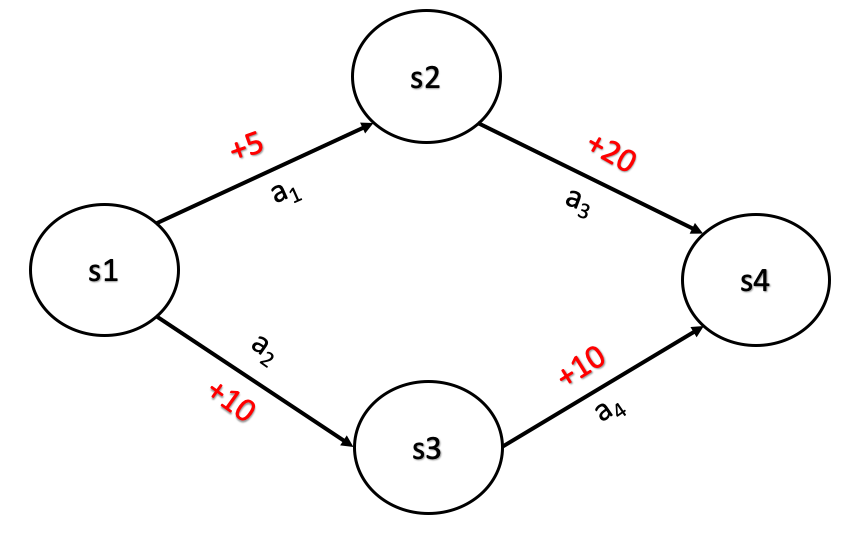
\includegraphics[width=0.6\textwidth]{figures/nonoptimal}
    \caption{Zero discount factor leads to non-optimal solution with s1-a2-s3-a4-s4. Discount factor greater than zero leads finds the optimal solution of s1-a1-s2-a3-s4 }
    \label{fig: nonoptimal}
\end{figure}

The value function is the expectation of returns, while an agent follows the policy (\(\pi\)). The policy represents the probability distribution of an agent taking action \(a\) in state \(s\). The policy is similar to the transition probability matrix in the Markov Chain section. Using policy, we can define the value function of an agent following the policy pi as below.
    \subsection{Q-Learning}

Q-learning algorithms have been the core of the RL research for almost 20 years. It combines the idea of TD learning in approximating action-value function. Through this approach, the computation converges faster than state-value approximation algorithms. Another strength of the Q-learning algorithm is its off-policy nature. The Q-learning agent can learn from the experiences of different policies. The off-policy nature makes the agent more data-efficient.

\begin{equation}
    Q(S_t, A_t) \longleftarrow Q(S_t, A_t) + \alpha [R_{t+1} + \gamma \max\limits_{a}Q(S_{t+1}, a)- Q(S_t, A_t))] 
\end{equation}

\section{Function Approximation}
As mentioned before, it is often impossible to find either the optimal policy or the optimal value function due to computational resources. It is often enough to find approximate solutions. Various function approximators are available for us to use. The main categorization follows as; linear and nonlinear function approximators. Their working principle is similar; they both follow a specific policy and sampling process. Based on the experiences, they approximate either policy or the value function. 
% by generalizing the states it has been over the states the agent has not been so far.

The application of neural networks provided RL methods a boost. Since the introduction of function approximators, the success of RL applications has increased significantly. Although function approximation tools bring convergency issues in some corner cases, it shows excellent success practically. 

The notation \(V(s)\) changes to \(V(s, w)\), if we define value function with weight parameterization. To find suitable weight parameters that represent the value function as general as possible, one needs to update parameters \(w\) at each step towards the smallest loss region based on a particular objective description. Firstly, we need to define an objective function and then find a method to tweak our weight parameters towards the objective gradually. 
There are a couple of possible objectives to learn in the literature; the state-value function, action-value function, or directly the policy.
In the case of the state value function, one can choose the objective function as the mean squared value loss between the estimated state-value function and the target state-value function (\ref{eqn:state-value}). While for policy approximation, expected return represents the objective function \ref{eqn:policy-objective}. 

Target state-value function can be the Monte-Carlo or TD target. Monte-Carlo’s target represents the expected return \((G_t)\), and TD target estimates the bootstrapped state-value function. The main difference between those targets is that Monte Carlo ensured to converge to a global optimum. In contrast, the bootstrapped TD target converges only to a local optimum near the global optimum. 

\begin{equation}
    \label{eqn:state-value}
    VE(w) = \sum\limits_{s\in S} \mu(s)[v_\pi(s) - \hat{v}(s,w)]^2
\end{equation}


Secondly, we need to optimize for the objective function. Optimaization is handled by the stochastic gradient descent method, it is the most used solution to improve the weight parameters based on a defined loss function. \ref{eqn:optimization} shows one gradient update step of the stochastic gradient descent method on the weight vector.  

\begin{equation}
    \label{eqn:optimization}
    w_{t+1} = w_t - \frac{1}{2}\alpha\nabla\Big[v_{\pi}(s) - \hat{v}(s,w)\Big]^2
\end{equation}

The optimal weight vector needs to find the right balance between strongly representing one state and generalizing to similar unseen states. As a result, our approximator needs to avoid either overfitting or underfitting.

% \subsection{Action Value Function Approximation}

One can also approximate action-value function in the same way as state-value function. The gradient update step of the action-value function is similar to the state-value function as in \ref{eqn:action_value}

\begin{equation}
    \label{eqn:action_value}
    w_{t+1} = w_t -\alpha\Big[U_t - \hat{q}(S_t,A_t, w_t)\Big]\nabla\hat{q}(S_t, A_t, w_t)
\end{equation}
\(U_t\) can be either TD or Monte Carlo target.

% \subsection{Policy Approximation}

So far, we have only considered the function approximation on the action and state functions.  Another promising and popular technique is to approximate the policy function directly. Policy function can lead us to optimal solution in a more direct way than action and state values. Since it directly aims to solve the problem at hand, to find the optimal policy \cite{SpinningUp2018}.
The objective function of policy gradient methods is simply the expectation of total return under policy \(\pi\).

\begin{equation}
    \label{eqn:policy-objective}
    J(\theta) = E\Big[\sum\limits_{t=0}^H R(s_t, u_t)\Big]
\end{equation}


\begin{equation}
    \theta \leftarrow \theta + \alpha\nabla_{\theta}J(\theta) 
\end{equation}
        \subsection{Neural Networks}
Neural networks are the unique case of function approximators. Although they follow the same procedure as SGD methods, their weight matrix is nonlinearly related to the approximated \(V(S_t,w_at)\). Nonlinear relation brings convergency issues and problems with instabilities. However, the practical success of these kinds of methods shadows the weak theoretical basis.

\begin{figure}[htbp]
    \centering
    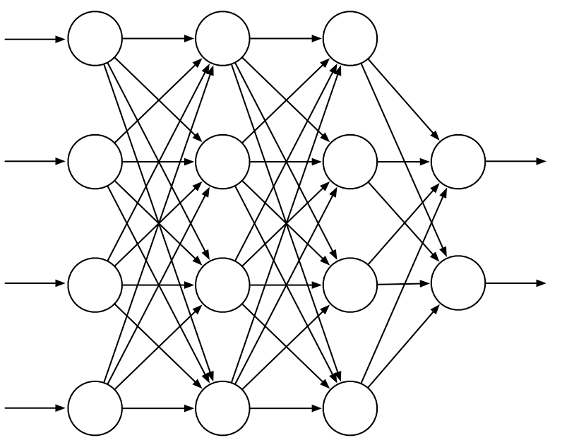
\includegraphics[width=0.4\textwidth]{figures/nn}
    \caption{Generic neural network with two hidden layers}
    \label{fig:nn}
\end{figure}

A generic neural network in \ref{fig:nn} comprises layers of artificial neurons connected with weight, bias vectors, and activation functions to each other. Each activation function feeds nonlinearity to the general equation. 

 

 


\section{Value-Based Reinforcement Learning}

Approximation of action-value or state-value function methods falls into the category of value-based RL. These methods are model-free, meaning that they use sampling to solve the optimal solution for the problem \cite{Mnih}. Simultaneously, they are off-policy algorithms, which makes them data efficient but high variance algorithms \cite{SpinningUp2018}. These methods only indirectly optimize the policy. Hence they are unstable during the learning phase \cite{Sutton2018}. Value function-based approaches can overestimate the policy's selected actions, which is a typical problem with Q-learning-based algorithms. 


\subsection{DQN}

DQN is the neural network extension of the Q-learning algorithm. It has shown that RL can handle high dimensional nonlinear control problems. DQN optimizes Bellman error by parameterizing the action-value function. Some extensions of DQN introduced experience replay buffer to cope with the high variance problem \cite{Lin1993}. \cite{Mnih}  inputs randomly collected mini-batches of experiences to the neural network consisting of multiple layers. Thanks to their neural network structure, they overcome the convergency issues.

\begin{equation}
    L(\theta) = E_{(s, a, r, s') \thicksim U(D)} \Big[\Big(r+ \gamma \max\limits_{a'}Q(s',a'; \theta^-)) - Q(s,a;\theta)\Big)^2\Big] 
\end{equation}


        \subsection{Extension of Q-networks}
        \subsection{Branch Dueeling Q-networks}
\section{Policy-Based RL}

Policy-based solutions directly parameterize the policy to find the optimal policy which returns the highest reward. These approaches proved to be more stable than Value-based counterparts. One reason behind stability is that actions are sampled from the continuous policy parameterization function, which outputs smooth action probabilities \cite{Sutton2018}. Similar to Value-based methods, policy-based RL also aims to solve the RL problem only with sampling in a model-free fashion.

\subsection{Policy Gradient}

Policy gradient methods incorporate stochastic gradient ascent on policy objective function. This update optimizes the \(\theta\) parameters of the policy. Unlike DQN, policy gradient methods perform each update in on-policy fashion. It uses only the experiences taken under the particular policy to update the parameters of this policy \cite{SpinningUp2018}.

\begin{align}
    \nabla J(\theta) \propto \sum\limits_s \mu(s) \sum\limits_a q_{\pi}(s,a)\nabla \pi(a | s, \theta)\\
    = E_{\pi} \Big[\sum\limits_a q_{\pi}(S_t,a)\nabla\pi(a | S_t, \theta)\Big]
\end{align}

        \subsection{Entropy-Based Approach}
        \subsection{Soft Actor Critic}
    % \subsection{Off-Policy RL}
    % \subsection{On-Policy RL}

% !TeX root = ../main.tex
% Add the above to each chapter to make compiling the PDF easier in some editors.

\section{Curriculum Learning}


One can gradually increase the level of the difficulty of a specific task to be learned to guide the training process and speed up the convergence time. Based on phycological studies, humans learn faster when they subject to the information in the form of a unique curriculum. That is because we are subjected to curriculum learning since they were toddlers. 



\section{State of Art}
    \subsection{Dexnet}
    \subsection{DQL Google}
